\section{R2U2 Software (C)}

\subsection{Process Overflow}
Figure \ref{fig:c_flow} shows the procedure of running the R2U2 C version by the user. From the high level, the user need to specify the MLTL formulas first. The formula will be converted into 1) binary instruction file; 2) SCQ size assignment file; 3) intervals for each temporal instruction. The user should also prepare the sensor trace file (*.trc) for verification.
\begin{figure}[H]
  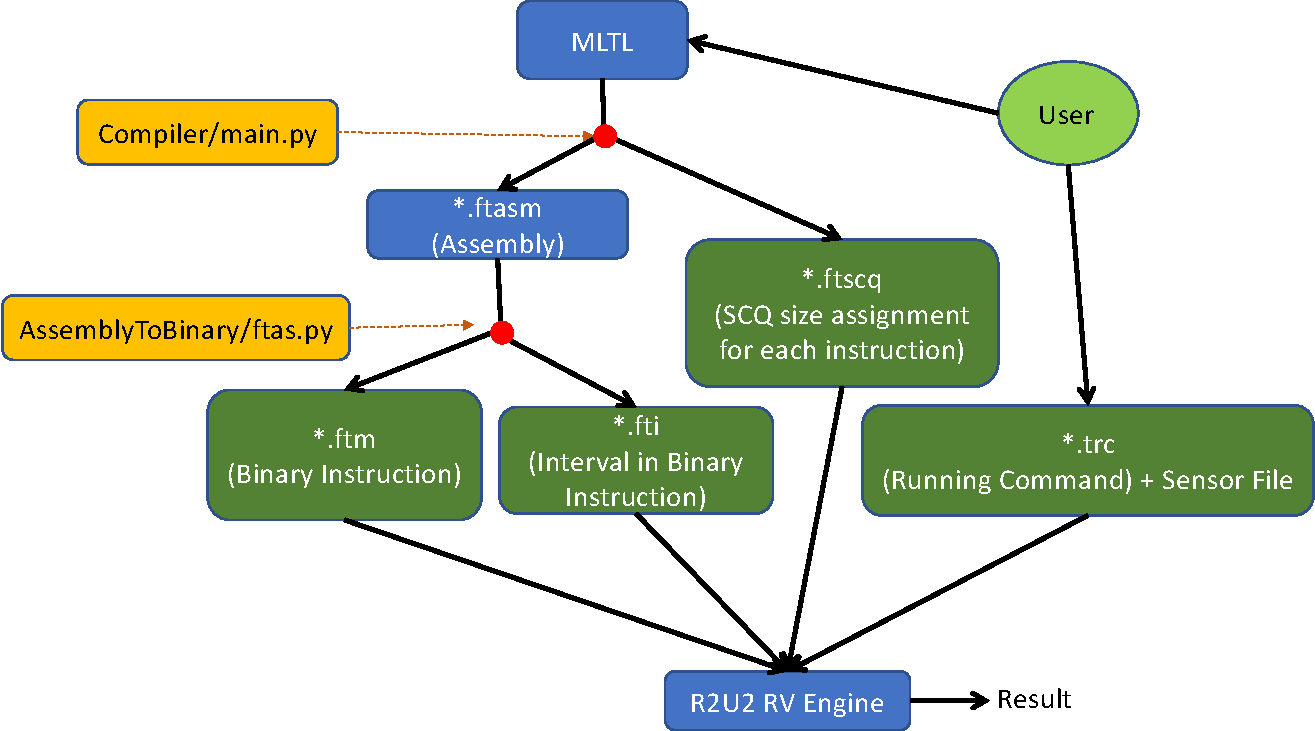
\includegraphics[scale=0.50]{fig/r2u2_c_flow.pdf}
  \caption{Deploying steps of R2U2 C. Blocks marked in green are the files required for the program execution. The yellow blocks tells the dependency of the tool scripts that handle the conversion.}
  \label{fig:c_flow}
\end{figure}

\subsection{R2U2 C Operation Modes and Trace Input Format}
There are two operation modes for R2U2 C: 1) Offline mode (regression test) 2) Online mode (embedded application).

To select the operation mode, comment/uncomment the line: \\
\colorbox{blue!30}{"\#define ONLINE\_MODE"} in \colorbox{gray!30}{r2u2/R2U2\_SW/R2U2\_C/src/R2U2.c}\\
and recompile the C program. Under different modes, the trace input is different (check Table \ref{tab:c_trace}).

\begin{table}[ht]
  \caption{Format and content of trace file}
  \label{tab:c_trace}
  \begin{center}
  \begin{tabular}{c|cccc|cccc}
      \hline
      Mode&\multicolumn{4}{c|}{Offline Mode}&\multicolumn{4}{c}{Online Mode}\\
      \cline{1-9}
      \multirow{1}{*}{Column Information}&sensor 0&sensor 1&sensor 2&\multicolumn{1}{c|}{...}&Command&sensor 0&sensor 1&...\\
      \hline
      \multirow{3}{*}{*.trc File Content}& 1.0 & 2.0 & 1.2 &...& -1 & 1.0 & 2.0 &...\\
      & 0.8 & 1.2 & 1.3 &...  & & & \\
      & 0.5 & 1.1 & 1.2 &... & & &  \\
      &...& & & ...& & & \\
      \hline
  \end{tabular}
  \end{center}
  \label{tab:multicol}
  \end{table}
Under the online mode, the command is included into the *.trc file. The trace file should be updated at each time stamp. In order to specify the behavior for R2U2, we use the first column in the trace file as the command to R2U2. The \textbf{command} variable can only be integers. If command=-2, R2U2 will terminate. If command=-1, R2U2 will reset the buffer and prepare for the new round of execution. The positive number of command represents the timestamp of the sensor value. Users should guarantee the timestamp will increase 1 by 1 starting from 0. Table \ref{tab:c_command_trace} summarizes the meaning of the \textbf{command} variable.
\begin{table}[h]
  \begin{tabularx}{\textwidth}{ |l|X| } 
   \hline
   Command Value & Description \\ 
   \hline
   -2 & Terminate the current execution. \\ 
   \hline
   -1 & Reset the instruction/data etc. buffer to restart the RV. Users must set command to -1 as the RV starts signal or the RV engine will not start.\\ 
   \hline
   i (Positive Integers) & Represent the sensor signal at time stamp i. The i should increase by 1 each time, starting from 0. (Increasing i tells the RV engine that new sensor value is coming.)\\
   \hline
   others & Unspecified\\
   \hline
  \end{tabularx}
  \caption{Meaning of `command' variable in *.trc file.}
  \label{tab:c_command_trace}
\end{table}


\subsection{Atomic Conversion Function}
% The sensor data in the *.trc file is the \colorbox{gray!30}{r2u2/R2U2\_SW/R2U2\_C/inputs/} folder.
Users need to manually specify the atomic conversion function. The function is specified in file: \\
\colorbox{gray!30}{r2u2/R2U2\_SW/R2U2\_C/src/AT/at\_conversion.c}. \\
Below is an example of the conversion function:
\begin{lstlisting}[language=C]
void at_checkers_update(const r2u2_input_data_t *r2u2_input_data){
	for (int i=0; i< N_ATOMICS; i++){
		atomics_vector[i] = AT_COMP((r2u2_input_data[i]), > , 0.5);
	}
}
\end{lstlisting}
,where \colorbox{blue!30}{atomics\_vector[i]} corresponds to atomic $a_i$ in the MLTL formula. \colorbox{blue!30}{r2u2\_input\_data[i]} corresponds to \textit{sensor i} in the trace file.
Uses can borrow some math marcos in \colorbox{gray!30}{at\_checkers.h} under the same folders or write their own math functions. 



\subsection{Command Line R2U2 C Execution}

\begin{table}[ht]
  \caption{Software dependency and the prerequisites}
  \label{tab:c_trace}
  \begin{center}
  \begin{tabular}{c|c}
      \hline
      \multirow{2}{*}{MLTL Compiler}& version $\geq$ python 3.0\\
      \cline{2-2}
      & ply; (pip install ply)\\
      \hline
      \multirow{2}{*}{R2U2 C}& pkg-config; (sudo apt install pkg-config)\\
      \cline{2-2}
      &  fftw3; (sudo apt-get install libfftw3-dev libfftw3-doc)\\
      \hline
  \end{tabular}
  \end{center}
  \label{tab:multicol}
  \end{table}

After determining the running mode and the trace file, now we can build the C project and check the execution output. Here is the steps for deploying the R2U2 C:
\begin{enumerate}
  \item Compile the C program:
    \begin{itemize}
      \item Navigate to the src folder
      \begin{lstlisting}[language=Bash]
      cd r2u2/R2U2-SW/R2U2_C/src/
      \end{lstlisting}
      \item Call MakeFile to compile
      \begin{lstlisting}[language=Bash]
      make
      \end{lstlisting}
    \end{itemize}

  \item Generate configuration files:
    \begin{itemize}
      \item Navigate to the tools/ folder:
      \begin{lstlisting}[language=Bash]
      cd r2u2/tools/
      \end{lstlisting}
      \item Convert MLTL formula to assembly:
      \begin{lstlisting}[language=Bash]
      python Compiler/main.py [MLTL formula]
      \end{lstlisting}
      This command will generate \textbf{tmp.ftasm} and \textbf{tmp.ftscq} configuration files.
      For the syntax of MLTL formula, refer to ??. (Note: special symbol (e.g., \&,$($,$)$,\textit{space}, etc.) should put a `\textbackslash' in the front).
      \item Convert assembly to binary text:
      \begin{lstlisting}[language=Bash]
      %#cat tmp.ftasm | python AssemblyToBinary/ftas.py tmp
      python AssemblyToBinary/ftas.py tmp.ftasm 4
      \end{lstlisting}
      This results the file \textbf{tmp.ftm} and \textbf{tmp.fti}.
    \end{itemize}

  \item Specify the trace file and start
  \begin{lstlisting}[language=Bash]
    bin/r2u2 [trace file *.trc]
  \end{lstlisting}
  If under online mode, then the user is in charge of updating the trace file at each time stamp.
\end{enumerate}

\clearpage
